\documentclass[a4paper, 10pt]{article}

\usepackage[utf8x]{inputenc}
\usepackage[english, russian, ukrainian]{babel}
\usepackage{cmap}

\usepackage{graphicx}
\usepackage{float}
\usepackage{amsmath}
\usepackage{listings}

\usepackage{geometry}
\geometry{top = 2cm}
\geometry{bottom = 2cm}
\geometry{left = 3cm}
\geometry{right = 1.5cm}

\begin{document}
\begin{titlepage}
\begin{center}
\large{
Міністерство освіти і науки, молоді та спорту України\\
Національний технічний університет України\\
``Київський політехнічний інститут''\\
Факультет прикладної математики\\
Кафедра спеціалізованих комп’ютерних систем\\
}

\vfill

\large{\bf{
Лабораторна робота №2\\
Дисципліна:\\
``Моделювання''\\
Тема:\\
``Моделювання динамічних систем в середовищі Simulink''\\
}}

\vfill

\begin{table}[h]
\centering
\begin{tabular}{lp{4cm}l}
Виконав:&&Перевірив:\\
Студент групи КВ--91&&Наливайчук М. В.\\
Євтушенко Є.О.&&\\
Залікова книжка № КВ--9105&&\\
\end{tabular}
\end{table}

\vfill

Київ \the\year
\end{center}
\end{titlepage}
\newpage

\section{Завдання}
Вивчити графічний інтерфейс Simulink. Навчиться моделювати скінченні динамічні систем в середовищі Simulink пакета MatLab.

\begin{enumerate}
\item Побудувати схеми рішення розглянутих задач в системі Simulink, отримати графік рішення. Порівняти з рішенням задач в MatLab за допомогою функції ode45. 
\item Розв’язати ці задачі в MatLab, побудувати графік рішень. 
\item{Побудувати схему рішення в Simulink і от отримати графік рішення наступних задач:}
	\begin{enumerate}
		\item{$
			\left\{\begin{array}{l}
				y'=\frac{z}{x},\\
				z'=\frac{2z^{2}}{x(y-1)}+\frac{z}{x},\quad\textrm{на [1, 2]}.\\
				y(1)=0,\quad z(1)=\frac{1}{3}\\
			\end{array}\right.
		$}

		\item{$
			\left\{\begin{array}{l}
				y'=(z-y)x,\\
				z'=(z+y)x,\quad\textrm{на [0, 1]}.\\
				y(0)=1,\quad z(0)=1\\
			\end{array}\right.
		$}

		\item{$
			\left\{\begin{array}{l}
				y'=cos(y+2z)+2,\\
				z'=\frac{2}{x+2y^{2}}+x+1,\quad\textrm{на [0, 0.3]}.\\
				y(0)=1,\quad z(0)=0.05\\
			\end{array}\right.
		$}

		\item{$
			\left\{\begin{array}{l}
				y'=e^{-(x^{2}+z^{2})}+2x,\\
				z'=2y^{2}+z,\quad\textrm{на [0, 0.3]}.\\
				y(0)=0.5,\quad z(0)=1\\
			\end{array}\right.
		$}

		\item{$y''=-\frac{y'}{x}+\frac{y}{x^{2}}+1,\quad y(3)=6,y'(3)=3.$}
	\end{enumerate}
\end{enumerate}

\section{Результати}
\begin{enumerate}
\item{
	Дано диференційне рівняння
	\begin{align*}
	&x'(t)+2x(t)=\sin(t),\\
	&x(0) = 0.
	\end{align*}

	\begin{figure}[H]
	\begin{center}
	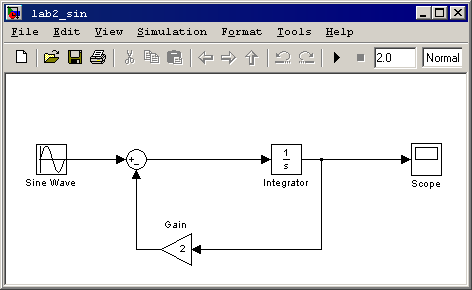
\includegraphics{1_sin_model.png}
	\caption{Схема рішення диференційного рівняння}
	\end{center}
	\end{figure}

	\begin{figure}[H]
	\begin{center}
	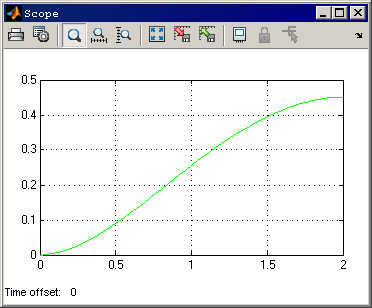
\includegraphics{1_sin.png}
	\caption{Рішення диференційного рівняння за допомогою Simulink}
	\end{center}
	\end{figure}

	\noindent
	f.m~-- функція--рішення диференційного рівняння.
	\begin{lstlisting}[numbers=left]
function sol=f(t);
    sol=(exp(-2*t)-cos(t)+2*sin(t))/5;
	\end{lstlisting}
	Її графік.
	\begin{lstlisting}[numbers=left]
t=(0:0.1:2);
y=f(t);
plot(t, y);
grid on;
	\end{lstlisting}

	\begin{figure}[H]
	\begin{center}
	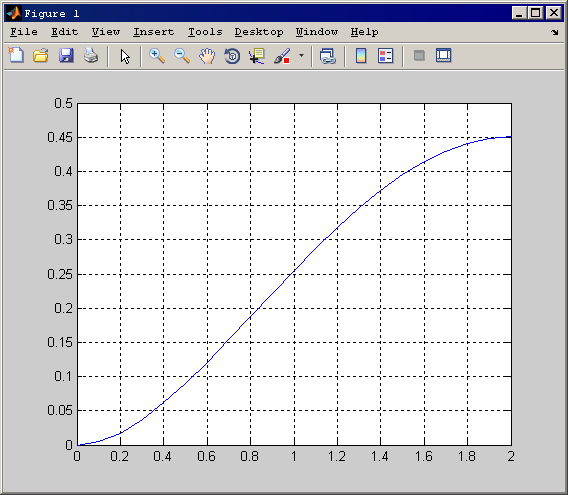
\includegraphics{1_sin_check.png}
	\caption{Графік функції--рішення диференційного рівняння}
	\end{center}
	\end{figure}

	\noindent
	xdiff.m~-- вхідна фунція для перевірки рішення за допомогою ode45.
	\begin{lstlisting}[numbers=left]
function dx = xdiff(t, x)
    dx = sin(t) - 2 * x;
end
	\end{lstlisting}

	Виклик функції: \texttt{ode45(@xdiff, [0 2], [0 0])}

	\begin{figure}[H]
	\begin{center}
	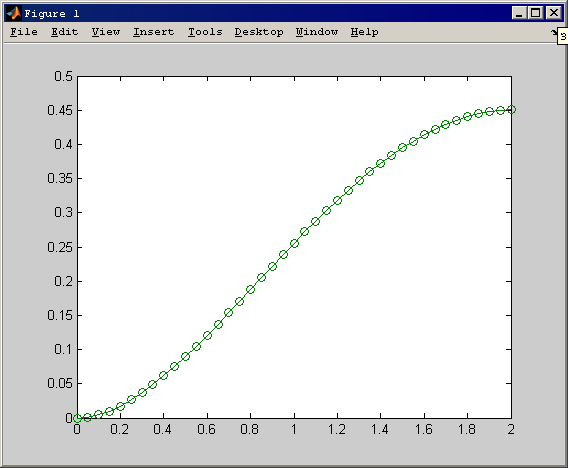
\includegraphics{1_ode45_sin.png}
	\caption{Графік функції--рішення диференційного рівняння, отриманого функцією ode45}
	\end{center}
	\end{figure}
}
\item{
	\begin{enumerate}
	\item{
		\begin{figure}[H]
		\begin{center}
		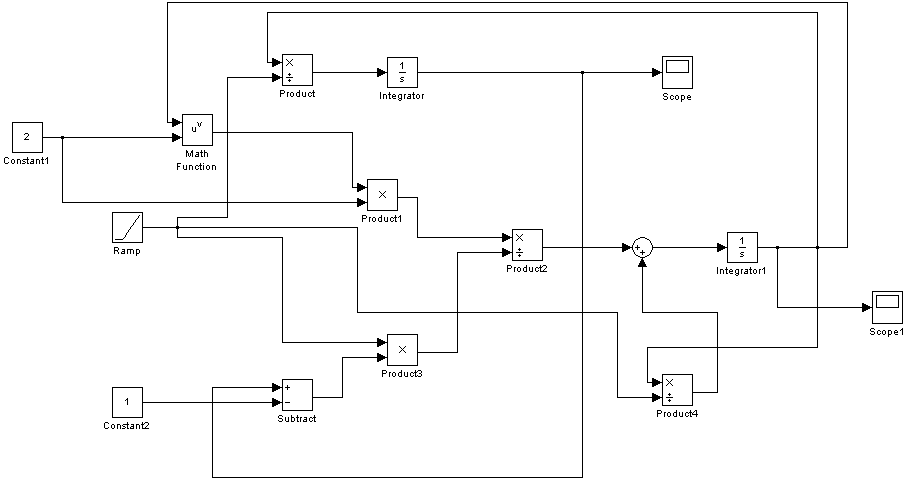
\includegraphics[angle=90]{lab2_1.png}
		\caption{Схема першої системи}
		\end{center}
		\end{figure}

		\begin{figure}[H]
		\begin{center}
		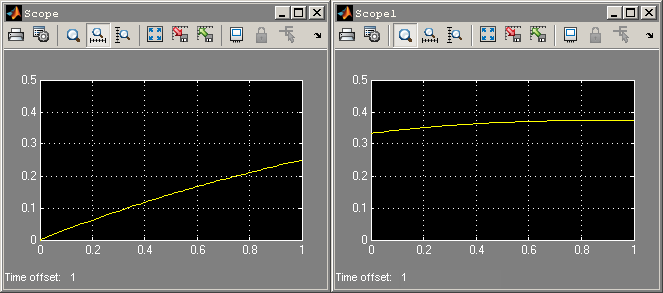
\includegraphics{lab2_1_sol.png}
		\caption{Рішення першої системи}
		\end{center}
		\end{figure}

		\noindent
		Функція для перевірки за допомогою ode45.
		\begin{lstlisting}[numbers=left]
function df = system1(x, f)
    % f(1) is y(x)
    % f(2) is z(x)
    df = zeros(2, 1);
    df(1) = f(2) / x;
    df(2) = 2 * (f(2))^2 / (x * (f(1) - 1)) + f(2) / x;
end
		\end{lstlisting}

		Виклик функції: \texttt{ode45(@system1, [1 2], [0 1/3])}

		\begin{figure}[H]
		\begin{center}
		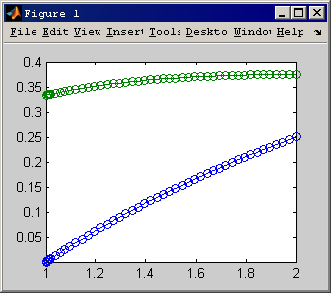
\includegraphics{lab2_1_ode45.png}
		\caption{Графік рішення системи диференційних рівняннь отриманий функцією ode45}
		\end{center}
		\end{figure}
	}
	\item{
		\begin{figure}[H]
		\begin{center}
		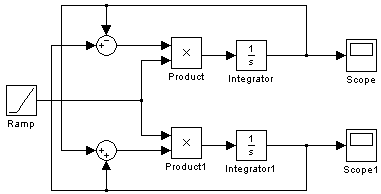
\includegraphics{lab2_2.png}
		\caption{Схема другої системи}
		\end{center}
		\end{figure}

		\begin{figure}[H]
		\begin{center}
		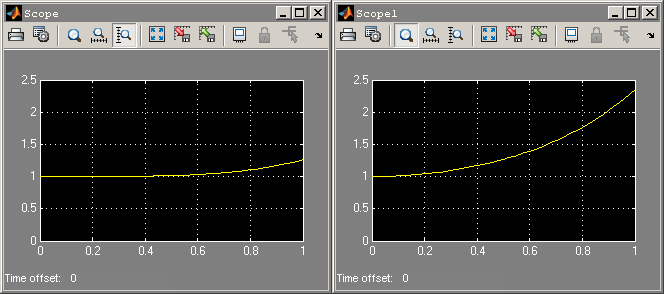
\includegraphics{lab2_2_sol.png}
		\caption{Рішення другої системи}
		\end{center}
		\end{figure}

		\noindent
		Функція для перевірки за допомогою ode45.
		\begin{lstlisting}[numbers=left]
function df = system2(x, f)
    % f(1) is y(x)
    % f(2) is z(x)
    df = zeros(2, 1);
    df(1) = (f(2) - f(1)) * x
    df(2) = (f(2) + f(1)) * x
end
		\end{lstlisting}

		Виклик функції: \texttt{ode45(@system2, [0 1], [1 1])}

		\begin{figure}[H]
		\begin{center}
		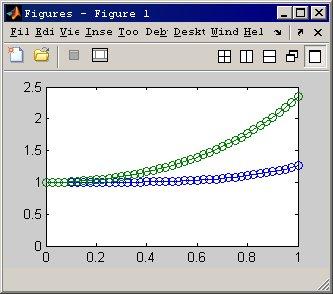
\includegraphics{lab2_2_ode45.png}
		\caption{Графік рішення системи диференційних рівняннь отриманий функцією ode45}
		\end{center}
		\end{figure}
	}
	\item{
		\begin{figure}[H]
		\begin{center}
		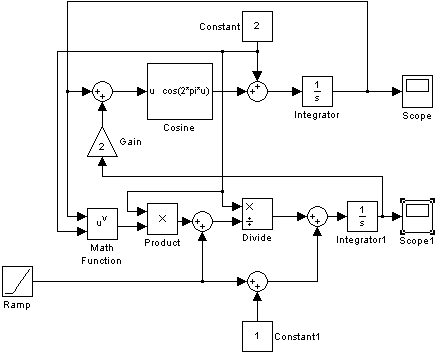
\includegraphics{lab2_3.png}
		\caption{Схема третьої системи}
		\end{center}
		\end{figure}

		\begin{figure}[H]
		\begin{center}
		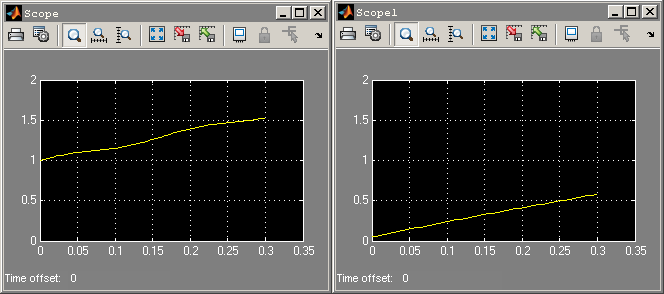
\includegraphics{lab2_3_sol.png}
		\caption{Рішення третьої системи}
		\end{center}
		\end{figure}

		\noindent
		Функція для перевірки за допомогою ode45.
		\begin{lstlisting}[numbers=left]
function df = system3(x, f)
    % f(1) is y(x)
    % f(2) is z(x)
    df = zeros(2, 1);
    df(1) = cos(f(1) + 2 * f(2)) + 2
    df(2) = 2 / (x + 2 * f(1)^2) + x + 1
end
		\end{lstlisting}

		Виклик функції: \texttt{ode45(@system3, [0 0.3], [1 0.05])}

		\begin{figure}[H]
		\begin{center}
		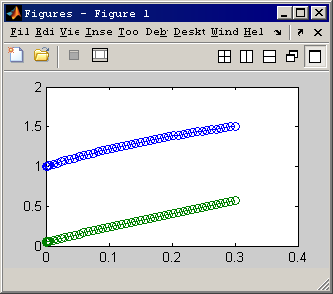
\includegraphics{lab2_3_ode45.png}
		\caption{Графік рішення системи диференційних рівняннь отриманий функцією ode45}
		\end{center}
		\end{figure}
	}
	\item{
		\begin{figure}[H]
		\begin{center}
		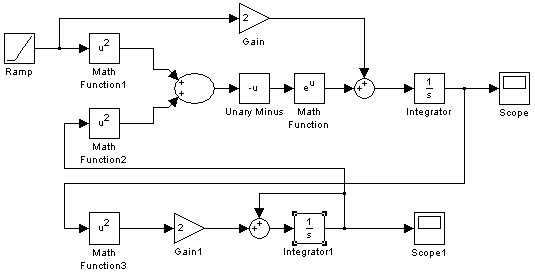
\includegraphics{lab2_4.png}
		\caption{Схема четвертої системи}
		\end{center}
		\end{figure}

		\begin{figure}[H]
		\begin{center}
		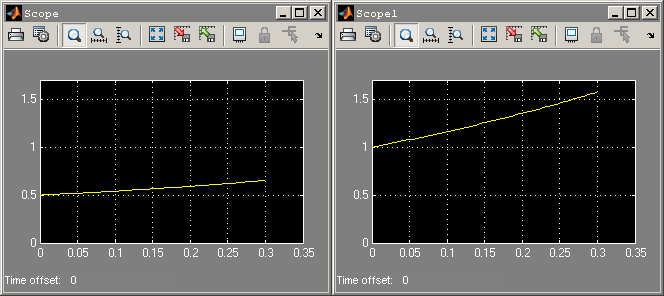
\includegraphics{lab2_4_sol.png}
		\caption{Рішення четвертої системи}
		\end{center}
		\end{figure}

		\noindent
		Функція для перевірки за допомогою ode45.
		\begin{lstlisting}[numbers=left]
function df = system4(x, f)
    % f(1) is y(x)
    % f(2) is z(x)
    df = zeros(2, 1);
    df(1) = exp(-(x^2 + f(2)^2)) + 2 * x
    df(2) = 2 * f(1)^2 + f(2)
end
		\end{lstlisting}

		Виклик функції: \texttt{ode45(@system4, [0 0.3], [0.5 1])}

		\begin{figure}[H]
		\begin{center}
		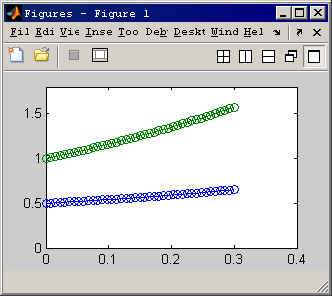
\includegraphics{lab2_4_ode45.png}
		\caption{Графік рішення системи диференційних рівняннь отриманий функцією ode45}
		\end{center}
		\end{figure}
	}
	\item{
		\begin{figure}[H]
		\begin{center}
		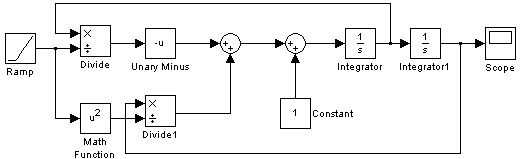
\includegraphics{lab2_5.png}
		\caption{Схема п'ятої системи}
		\end{center}
		\end{figure}

		\begin{figure}[H]
		\begin{center}
		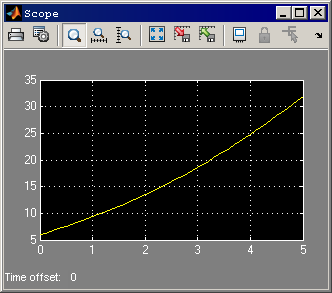
\includegraphics{lab2_5_sol.png}
		\caption{Рішення п'ятої системи}
		\end{center}
		\end{figure}

		\noindent
		Функція для перевірки за допомогою ode45.
		\begin{lstlisting}[numbers=left]
function df = system5(x, f)
    % f(1) is y'(x)
    % f(2) is y(x)
    df = zeros(2, 1);
    df(2) = -f(1) / x + f(2) / (x^2) + 1
    df(1) = f(1)
end
		\end{lstlisting}

		Виклик функції: \texttt{ode45(@system5, [3 4], [3 6])}

		\begin{figure}[H]
		\begin{center}
		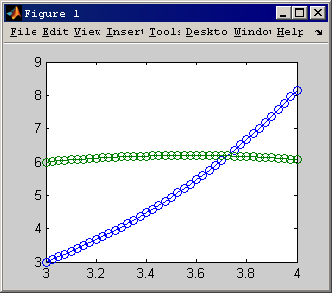
\includegraphics{lab2_5_ode45.png}
		\caption{Графік рішення системи диференційних рівняннь отриманий функцією ode45}
		\end{center}
		\end{figure}
	}
	\end{enumerate}
}
\end{enumerate}
\end{document}
